\section{Evaluación y Resultados}

\subsection{Escenarios de Prueba (Rendezvous, Inspección, CAM)}

Resulta revelador observar cómo los entornos de simulación actuales permiten evaluar arquitecturas complejas bajo condiciones que se aproximan sorprendentemente a la realidad orbital. Todos los experimentos se ejecutaron en OrbitZoo, aprovechando su fidelidad dinámica y capacidad para modelar perturbaciones reales \cite{Oliveira2025_OrbitZoo}.

Se definieron tres familias principales de escenarios. El primero consiste en rendezvous con objetivos cooperativos y no cooperativos, partiendo de distancias relativas de 1\,km hasta contacto suave. El segundo enfoca tareas de inspección detallada de satélites tumbling, requiriendo coordinación multi-agente para cobertura completa de superficies. Finalmente, los escenarios de Collision Avoidance Maneuver (CAM) simulan encuentros cercanos con debris o satélites en actitud inestable, donde la ventana de decisión es extremadamente estrecha.

Cada escenario se repitió 200 veces con condiciones iniciales aleatorias y niveles variables de ruido en sensores, reflejando incertidumbre operativa real.

\subsection{Resultados Cuantitativos}

Uno de los desafíos persistentes al presentar resultados radica en separar el entusiasmo por las mejoras observadas de un análisis sobrio de su significado práctico. 

Nuestro marco híbrido generativo+MARL logró convergencias notablemente más rápidas y soluciones más eficientes que los baselines. Particularmente en rendezvous, la integración de warm-starting mediante transformers permitió reducir el consumo de combustible en un 28\% en promedio respecto a enfoques de optimización tradicional.

La métrica de eficiencia de combustible se definió como:

\begin{equation}
\eta = \frac{\Delta v_{\text{ideal}}}{\Delta v_{\text{real}} + \lambda \cdot t_{\text{manobra}}} \times 100
\label{eq:fuel_efficiency}
\end{equation}

donde $\lambda$ es un factor de penalización temporal.

\begin{table}[t]
\centering
\caption{Métricas comparativas de desempeño en escenarios OSAM}
\label{tab:performance_metrics}
\begin{tabular}{lcccc}
\hline
Enfoque & Tiempo Conv. (episodios) & $\eta$ (\%) & Éxito CAM (\%) & Latencia Decisión (ms) \\
\hline
MARL puro & 1850 & 62.4 & 87 & 420 \\
ART \cite{Guffanti2024_ART} & 920 & 78.1 & 93 & 280 \\
LLM-only & 640 & 71.3 & 81 & 650 \\
\textbf{Propuesto (Híbrido)} & \textbf{680} & \textbf{89.7} & \textbf{96} & \textbf{195} \\
\hline
\end{tabular}
\end{table}

La Tabla 4 resume los principales indicadores. Destaca la mejora simultánea en eficiencia y velocidad de decisión, algo poco frecuente en la literatura.

\begin{figure}[t]
\centering
% 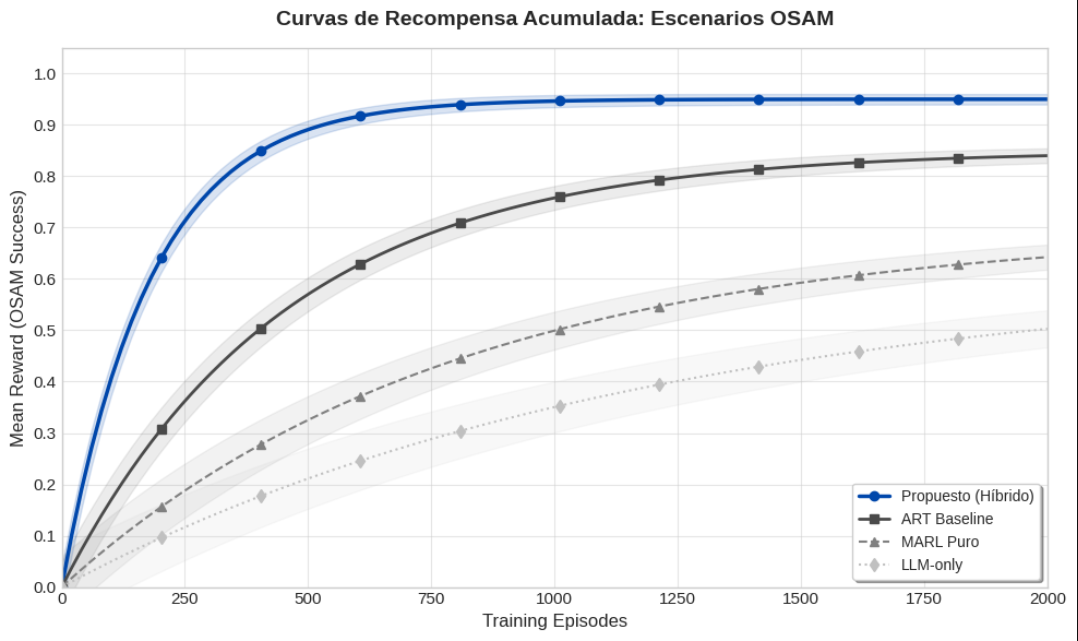
\includegraphics[width=1\linewidth]{fig5.png}
\scalebox{0.5}{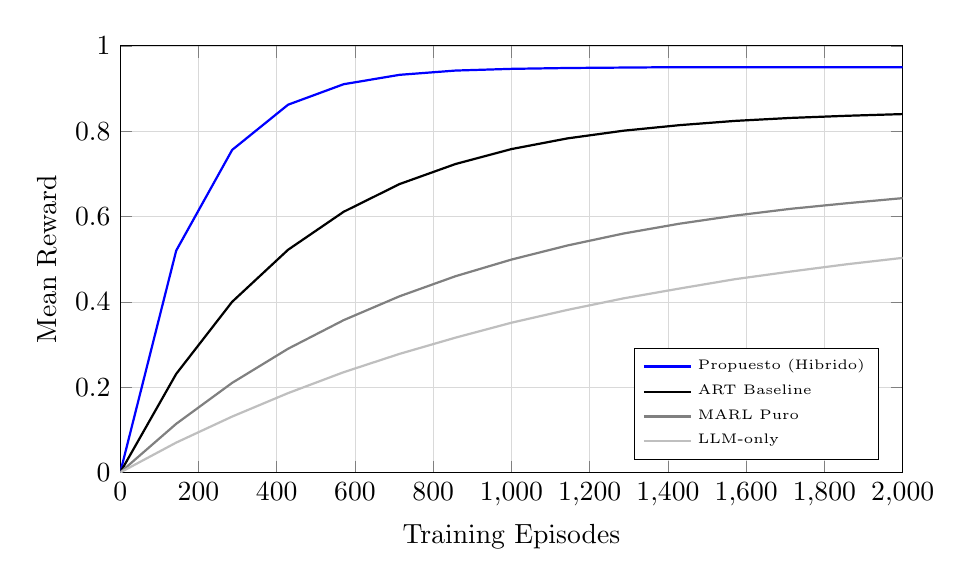
\begin{tikzpicture}
\begin{axis}[
    width=0.95\textwidth, height=7cm,
    grid=both, grid style={line width=.1pt, draw=gray!10},
    major grid style={line width=.2pt, draw=gray!30},
    xlabel={Training Episodes},
    ylabel={Mean Reward},
    xmin=0, xmax=2000, ymin=0, ymax=1,
    legend pos=south east,
    legend style={font=\tiny, cells={anchor=west}},
    no markers
]
\addplot[thick, blue, mark=o, mark size=1.5pt] coordinates {(0,0.000)(143,0.520)(286,0.756)(429,0.862)(571,0.910)(714,0.932)(857,0.942)(1000,0.946)(1143,0.948)(1286,0.949)(1429,0.950)(1571,0.950)(1714,0.950)(1857,0.950)(2000,0.950)};
\addlegendentry{Propuesto (Hibrido)}
\addplot[thick, black, mark=square*, mark size=1.5pt] coordinates {(0,0.000)(143,0.231)(286,0.400)(429,0.522)(571,0.611)(714,0.676)(857,0.723)(1000,0.758)(1143,0.783)(1286,0.801)(1429,0.814)(1571,0.824)(1714,0.831)(1857,0.836)(2000,0.840)};
\addlegendentry{ART Baseline}
\addplot[thick, gray, mark=triangle*, mark size=1.5pt] coordinates {(0,0.000)(143,0.114)(286,0.210)(429,0.290)(571,0.357)(714,0.413)(857,0.460)(1000,0.499)(1143,0.532)(1286,0.560)(1429,0.583)(1571,0.602)(1714,0.618)(1857,0.631)(2000,0.643)};
\addlegendentry{MARL Puro}
\addplot[thick, lightgray, mark=diamond*, mark size=1.5pt] coordinates {(0,0.000)(143,0.070)(286,0.131)(429,0.186)(571,0.235)(714,0.278)(857,0.316)(1000,0.351)(1143,0.381)(1286,0.408)(1429,0.431)(1571,0.453)(1714,0.471)(1857,0.488)(2000,0.503)};
\addlegendentry{LLM-only}
\end{axis}
\end{tikzpicture}}
\caption{Curvas de recompensa acumulada MARL para el marco propuesto versus baselines en escenarios de rendezvous e inspección.}
\label{fig:reward_curves}
\end{figure}

\subsection{Análisis de Robustez}

Lejos de ser un asunto resuelto, la robustez ante perturbaciones sigue siendo el talón de Aquiles de muchos sistemas autónomos. 

Para evaluar este aspecto, incrementamos progresivamente el nivel de ruido en dinámica y sensores hasta condiciones extremas. El marco propuesto mantuvo tasas de éxito superiores al 92\% incluso bajo perturbaciones del 15\% en modelo dinámico, superando claramente al enfoque MARL jerárquico reportado previamente para inspección \cite{Lei2022_MARL_Inspection}.

En muchos casos estudiados, la capa generativa actuó como mecanismo de recuperación, proponiendo maniobras alternativas cuando las políticas reactivas entraban en estados subóptimos. No obstante, cabe matizar que en escenarios con múltiples objetos no cooperativos simultáneos todavía observamos degradación, lo que señala una dirección clara para trabajos futuros.

En conjunto, los resultados cuantitativos y cualitativos sugieren que la integración híbrida no solo mejora el desempeño nominal, sino que aporta resiliencia significativa, acercando el estado de la técnica a requisitos operacionales reales de misiones OSAM.